%% Created by Maple 2020.1, Windows 10
%% Source Worksheet: workshop1
%% Generated: Sun Dec 06 17:06:32 CET 2020
\documentclass{article}
\usepackage{amssymb}
\usepackage{graphicx}
\usepackage{hyperref}
\usepackage{listings}
\usepackage{maplestd2e}
\usepackage[utf8]{inputenc}
\begin{document}
\lstset{basicstyle=\ttfamily,breaklines=true,columns=flexible}
\pagestyle{empty}
\DefineParaStyle{Maple Bullet Item}
\DefineParaStyle{Maple Heading 1}
\DefineParaStyle{Maple Warning}
\DefineParaStyle{Maple Heading 4}
\DefineParaStyle{Maple Heading 2}
\DefineParaStyle{Maple Heading 3}
\DefineParaStyle{Maple Dash Item}
\DefineParaStyle{Maple Error}
\DefineParaStyle{Maple Title}
\DefineParaStyle{Maple Text Output}
\DefineParaStyle{Maple Normal}
\DefineCharStyle{Maple 2D Output}
\DefineCharStyle{Maple 2D Input}
\DefineCharStyle{Maple Maple Input}
\DefineCharStyle{Maple 2D Math}
\DefineCharStyle{Maple Hyperlink}
\begin{Maple Normal}{
\mapleinline{inert}{2d}{with(combinat); -1}{\[\]}
}\end{Maple Normal}
\begin{Maple Normal}{
\mapleinline{inert}{2d}{}{\[\]}
}\end{Maple Normal}
\section{\textbf{Workshop 1 - Sociale netværk}}
\begin{Maple Normal}{
En gruppe mennesker er ved at opstarte et nyt socialt medie og gør sig\linebreak
nogle overvejelser om, hvordan det skal fungere. Indtil videre er mængden af\linebreak
brugere på mediet givet ved}\end{Maple Normal}

\begin{Maple Normal}{
\mapleinline{inert}{2d}{}{\[\]}
}\end{Maple Normal}
\begin{Maple Normal}{
\mapleinline{inert}{2d}{Typesetting:-mrow(Typesetting:-mi("A", italic = "true", mathvariant = "italic"), Typesetting:-mo("=", mathvariant = "normal", fence = "false", separator = "false", stretchy = "false", symmetric = "false", largeop = "false", movablelimits = "false", accent = "false", lspace = "0.2777778em", rspace = "0.2777778em"), Typesetting:-mfenced(Typesetting:-mrow(Typesetting:-mi("Tom", italic = "true", mathvariant = "italic"), Typesetting:-mo(",", mathvariant = "normal", fence = "false", separator = "true", stretchy = "false", symmetric = "false", largeop = "false", movablelimits = "false", accent = "false", lspace = "0.0em", rspace = "0.3333333em"), Typesetting:-mo(" ", mathvariant = "normal", fence = "false", separator = "false", stretchy = "false", symmetric = "false", largeop = "false", movablelimits = "false", accent = "false", lspace = "0.0em", rspace = "0.0em"), Typesetting:-mi("Mia", italic = "true", mathvariant = "italic"), Typesetting:-mo(",", mathvariant = "normal", fence = "false", separator = "true", stretchy = "false", symmetric = "false", largeop = "false", movablelimits = "false", accent = "false", lspace = "0.0em", rspace = "0.3333333em"), Typesetting:-mo(" ", mathvariant = "normal", fence = "false", separator = "false", stretchy = "false", symmetric = "false", largeop = "false", movablelimits = "false", accent = "false", lspace = "0.0em", rspace = "0.0em"), Typesetting:-mi("Bob", italic = "true", mathvariant = "italic"), Typesetting:-mo(",", mathvariant = "normal", fence = "false", separator = "true", stretchy = "false", symmetric = "false", largeop = "false", movablelimits = "false", accent = "false", lspace = "0.0em", rspace = "0.3333333em"), Typesetting:-mo(" ", mathvariant = "normal", fence = "false", separator = "false", stretchy = "false", symmetric = "false", largeop = "false", movablelimits = "false", accent = "false", lspace = "0.0em", rspace = "0.0em"), Typesetting:-mi("Liv", italic = "true", mathvariant = "italic"), Typesetting:-mo(",", mathvariant = "normal", fence = "false", separator = "true", stretchy = "false", symmetric = "false", largeop = "false", movablelimits = "false", accent = "false", lspace = "0.0em", rspace = "0.3333333em"), Typesetting:-mo(" ", mathvariant = "normal", fence = "false", separator = "false", stretchy = "false", symmetric = "false", largeop = "false", movablelimits = "false", accent = "false", lspace = "0.0em", rspace = "0.0em"), Typesetting:-mi("Kim", italic = "true", mathvariant = "italic"), Typesetting:-mo(",", mathvariant = "normal", fence = "false", separator = "true", stretchy = "false", symmetric = "false", largeop = "false", movablelimits = "false", accent = "false", lspace = "0.0em", rspace = "0.3333333em"), Typesetting:-mo(" ", mathvariant = "normal", fence = "false", separator = "false", stretchy = "false", symmetric = "false", largeop = "false", movablelimits = "false", accent = "false", lspace = "0.0em", rspace = "0.0em"), Typesetting:-mi("Noa", italic = "true", mathvariant = "italic"), Typesetting:-mo(",", mathvariant = "normal", fence = "false", separator = "true", stretchy = "false", symmetric = "false", largeop = "false", movablelimits = "false", accent = "false", lspace = "0.0em", rspace = "0.3333333em"), Typesetting:-mo(" ", mathvariant = "normal", fence = "false", separator = "false", stretchy = "false", symmetric = "false", largeop = "false", movablelimits = "false", accent = "false", lspace = "0.0em", rspace = "0.0em"), Typesetting:-mi("Gry", italic = "true", mathvariant = "italic")), mathvariant = "normal", open = "{", close = "}"), Typesetting:-mo(".", mathvariant = "normal", fence = "false", separator = "false", stretchy = "false", symmetric = "false", largeop = "false", movablelimits = "false", accent = "false", lspace = "0.0em", rspace = "0.0em"))}{\[A =\left({\it Tom} ,\mathop{\rm  }{\it Mia} ,\mathop{\rm  }{\it Bob} ,\mathop{\rm  }{\it Liv} ,\mathop{\rm  }{\it Kim} ,\mathop{\rm  }{\it Noa}\\
\mbox{} ,\mathop{\rm  }{\it Gry} \right).\]}
}\end{Maple Normal}
\begin{Maple Normal}{
}\end{Maple Normal}
\begin{Maple Normal}{
Som udgangspunkt er det lavet sådan, at man kan følge andre brugere (lige-\linebreak
som på f.eks. Instagram og Twitter). Dette giver anledning til en relation på\linebreak
A sådan at (a, b) ∈ R (også skrevet aRb) hvis person a følger person b. På\linebreak
Figur 1 er illustreret, hvem der følger hvem på nuværende tidspunkt (som\linebreak
udgangspunkt følger man sig selv, da man kan se sine egne opslag).}\end{Maple Normal}

\begin{Maple Normal}{
\mapleinline{inert}{2d}{}{\[\]}
}\end{Maple Normal}
\begin{Maple Normal}{
\raisebox{9.166666666666666in}{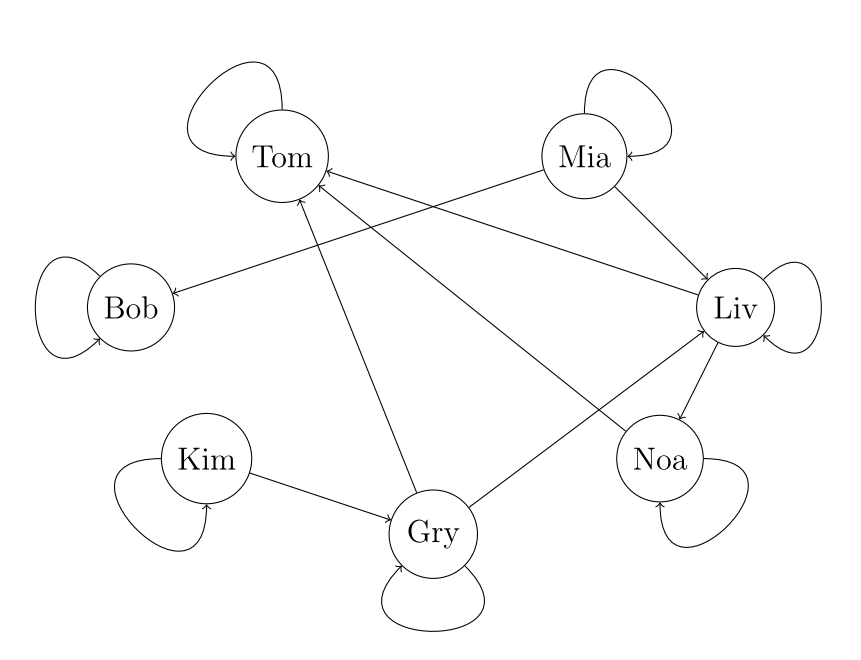
\includegraphics[keepaspectratio,height=9.166666666666666in]{workshop1_image0.png}}}\end{Maple Normal}
\begin{Maple Normal}{
\mapleinline{inert}{2d}{}{\[\]}
}\end{Maple Normal}
\begin{Maple Normal}{
Figure 1: En pil fra en person til en anden betyder, at den første person\linebreak
følger den anden. F.eks. gælder det, at Mia følger Bob.}\end{Maple Normal}

\begin{Maple Normal}{
}\end{Maple Normal}
\begin{Maple Normal}{
}\end{Maple Normal}
\begin{Maple Normal}{
}\end{Maple Normal}
\subsection{\textbf{Delopgave 1}}
\subsubsection{\textbf{\textit{1. }}}
\begin{Maple Normal}{
\textbf{Opskriv relatiionen beskrevet ovenfor og vist i Figur 1}}\end{Maple Normal}

\begin{Maple Normal}{
}\end{Maple Normal}
\begin{Maple Normal}{
Som man får beskrevet "Dette giver anledning til en relation på A sådan at (a, b) ∈ R (også skrevet aRb) hvis person a følger person b". Dvs. at hvis Mia følger Bob, så er \mapleinline{inert}{2d}{`in`(Mia, Bob, R)}{$\displaystyle {it in}\left({\it Mia},{\it Bob},R\right)$}
. På figur et kan alle disse aflæses og man får følgende:}\end{Maple Normal}

\begin{Maple Normal}{
\mapleinline{inert}{2d}{R = {Bob, Gry, Kim, Liv, Mia, Noa, Tom}}{$\displaystyle R= \left\{ {\it Bob},{\it Gry},{\it Kim},{\it Liv},{\it Mia}\\
\mbox{},{\it Noa},{\it Tom} \right\} $}
\mapleinline{inert}{2d}{}{$\displaystyle $}
}\end{Maple Normal}
\begin{Maple Normal}{
\mapleinline{inert}{2d}{}{$\displaystyle $}
\mapleinline{inert}{2d}{}{$\displaystyle $}
}\end{Maple Normal}
\subsubsection{\textbf{\textit{2. }}}
\begin{Maple Normal}{
\textbf{Hvad er kardinaliteten af relationen?}}\end{Maple Normal}

\begin{Maple Normal}{
}\end{Maple Normal}
\begin{Maple Normal}{
Kardinaliteten er antallet af elementer i mængden. Vi har her at hvert par er et element.}\end{Maple Normal}

\begin{Maple Normal}{
}\end{Maple Normal}
\begin{Maple Normal}{
Tæller man elementerne kommer man frem til at \mapleinline{inert}{2d}{abs(R) = 15.}{$\displaystyle  \left| R \right| = 15.0$}
}\end{Maple Normal}

\begin{Maple Normal}{
\mapleinline{inert}{2d}{}{\[\]}
}\end{Maple Normal}
\subsubsection{\textbf{\textit{3. }}\mapleinline{inert}{2d}{}{$\displaystyle $}
}
\begin{Maple Normal}{
\textbf{Relationen kan også beskrives som en delmængde af et kartesisk produkt.\linebreak
}\textbf{Hvilket kartesisk produkt er der tale om, og hvad er kardinaliteten af\linebreak
}\textbf{det?}}\end{Maple Normal}

\begin{Maple Normal}{
}\end{Maple Normal}
\begin{Maple Normal}{
Hvis man kigger på mængden \mapleinline{inert}{2d}{Typesetting:-mrow(Typesetting:-mi("A", italic = "true", mathvariant = "italic"), Typesetting:-mo("=", mathvariant = "normal", fence = "false", separator = "false", stretchy = "false", symmetric = "false", largeop = "false", movablelimits = "false", accent = "false", lspace = "0.2777778em", rspace = "0.2777778em"), Typesetting:-mfenced(Typesetting:-mrow(Typesetting:-mi("Tom", italic = "true", mathvariant = "italic"), Typesetting:-mo(",", mathvariant = "normal", fence = "false", separator = "true", stretchy = "false", symmetric = "false", largeop = "false", movablelimits = "false", accent = "false", lspace = "0.0em", rspace = "0.3333333em"), Typesetting:-mo(" ", mathvariant = "normal", fence = "false", separator = "false", stretchy = "false", symmetric = "false", largeop = "false", movablelimits = "false", accent = "false", lspace = "0.0em", rspace = "0.0em"), Typesetting:-mi("Mia", italic = "true", mathvariant = "italic"), Typesetting:-mo(",", mathvariant = "normal", fence = "false", separator = "true", stretchy = "false", symmetric = "false", largeop = "false", movablelimits = "false", accent = "false", lspace = "0.0em", rspace = "0.3333333em"), Typesetting:-mo(" ", mathvariant = "normal", fence = "false", separator = "false", stretchy = "false", symmetric = "false", largeop = "false", movablelimits = "false", accent = "false", lspace = "0.0em", rspace = "0.0em"), Typesetting:-mi("Bob", italic = "true", mathvariant = "italic"), Typesetting:-mo(",", mathvariant = "normal", fence = "false", separator = "true", stretchy = "false", symmetric = "false", largeop = "false", movablelimits = "false", accent = "false", lspace = "0.0em", rspace = "0.3333333em"), Typesetting:-mo(" ", mathvariant = "normal", fence = "false", separator = "false", stretchy = "false", symmetric = "false", largeop = "false", movablelimits = "false", accent = "false", lspace = "0.0em", rspace = "0.0em"), Typesetting:-mi("Liv", italic = "true", mathvariant = "italic"), Typesetting:-mo(",", mathvariant = "normal", fence = "false", separator = "true", stretchy = "false", symmetric = "false", largeop = "false", movablelimits = "false", accent = "false", lspace = "0.0em", rspace = "0.3333333em"), Typesetting:-mo(" ", mathvariant = "normal", fence = "false", separator = "false", stretchy = "false", symmetric = "false", largeop = "false", movablelimits = "false", accent = "false", lspace = "0.0em", rspace = "0.0em"), Typesetting:-mi("Kim", italic = "true", mathvariant = "italic"), Typesetting:-mo(",", mathvariant = "normal", fence = "false", separator = "true", stretchy = "false", symmetric = "false", largeop = "false", movablelimits = "false", accent = "false", lspace = "0.0em", rspace = "0.3333333em"), Typesetting:-mo(" ", mathvariant = "normal", fence = "false", separator = "false", stretchy = "false", symmetric = "false", largeop = "false", movablelimits = "false", accent = "false", lspace = "0.0em", rspace = "0.0em"), Typesetting:-mi("Noa", italic = "true", mathvariant = "italic"), Typesetting:-mo(",", mathvariant = "normal", fence = "false", separator = "true", stretchy = "false", symmetric = "false", largeop = "false", movablelimits = "false", accent = "false", lspace = "0.0em", rspace = "0.3333333em"), Typesetting:-mo(" ", mathvariant = "normal", fence = "false", separator = "false", stretchy = "false", symmetric = "false", largeop = "false", movablelimits = "false", accent = "false", lspace = "0.0em", rspace = "0.0em"), Typesetting:-mi("Gry", italic = "true", mathvariant = "italic")), mathvariant = "normal", open = "{", close = "}"), Typesetting:-mo(".", mathvariant = "normal", fence = "false", separator = "false", stretchy = "false", symmetric = "false", largeop = "false", movablelimits = "false", accent = "false", lspace = "0.0em", rspace = "0.0em"))}{$\displaystyle A =\left({\it Tom} ,\mathop{\rm  }{\it Mia} ,\mathop{\rm  }{\it Bob} ,\mathop{\rm  }{\it Liv} ,\mathop{\rm  }{\it Kim} ,\mathop{\rm  }{\it Noa}\\
\mbox{} ,\mathop{\rm  }{\it Gry} \right).$}
 Finder man det kartesiske produkt \mapleinline{inert}{2d}{Typesetting:-delayCrossProduct(A, A)}{$\displaystyle {\it delayCrossProduct} \left( A,A \right) $}
 får man alle mængde svarende til at alle følger hinanden.}\end{Maple Normal}

\begin{Maple Normal}{
}\end{Maple Normal}
\begin{Maple Normal}{
\mapleinline{inert}{2d}{A := {Bob, Gry, Kim, Liv, Mia, Noa, Tom}; -1}{\[\]}
}\end{Maple Normal}
\begin{Maple Normal}{
}\end{Maple Normal}
\begin{Maple Normal}{
\mapleinline{inert}{2d}{T := cartprod([A, A]); -1}{\[\]}
}\end{Maple Normal}
\begin{Maple Normal}{
\mapleinline{inert}{2d}{while not T[finished] do T[nextvalue]() end do; -1}{\[\]}
}\end{Maple Normal}
\begin{Maple Normal}{
Denne mængde svarer til at alle følger alle. I relation sker dette ikke, men alle par som er i relation er også i \mapleinline{inert}{2d}{Typesetting:-delayCrossProduct(A, A) = A^2}{$\displaystyle {\it delayCrossProduct} \left( A,A \right) ={A}^{2}$}
. Derfor må det gælde at \mapleinline{inert}{2d}{R subset A^2}{$\displaystyle R \subseteq {A}^{2}$}
}\end{Maple Normal}

\begin{Maple Normal}{
\mapleinline{inert}{2d}{}{\[\]}
}\end{Maple Normal}
\begin{Maple Normal}{
\mapleinline{inert}{2d}{}{\[\]}
}\end{Maple Normal}
\begin{Maple Normal}{
Kardinaliteten af et kartesisk produkt ur givet ved \mapleinline{inert}{2d}{Typesetting:-mrow(Typesetting:-mfenced(Typesetting:-mrow(Typesetting:-mi("A", italic = "true", mathvariant = "italic"), Typesetting:-mo("&times;", mathvariant = "normal", fence = "false", separator = "false", stretchy = "false", symmetric = "false", largeop = "false", movablelimits = "false", accent = "false", lspace = "0.2222222em", rspace = "0.2222222em"), Typesetting:-mi("B", italic = "true", mathvariant = "italic")), mathvariant = "normal", open = "|", close = "|"), Typesetting:-mo("=", mathvariant = "normal", fence = "false", separator = "false", stretchy = "false", symmetric = "false", largeop = "false", movablelimits = "false", accent = "false", lspace = "0.2777778em", rspace = "0.2777778em"), Typesetting:-mo("|", mathvariant = "normal", fence = "false", separator = "false", stretchy = "true", symmetric = "false", largeop = "false", movablelimits = "false", accent = "false", lspace = "0.1111111em", rspace = "0.1111111em"), Typesetting:-mi("A", italic = "true", mathvariant = "italic"), Typesetting:-mo("|", mathvariant = "normal", fence = "false", separator = "false", stretchy = "true", symmetric = "false", largeop = "false", movablelimits = "false", accent = "false", lspace = "0.1111111em", rspace = "0.1111111em"), Typesetting:-mo("&sdot;", mathvariant = "normal", fence = "false", separator = "false", stretchy = "false", symmetric = "false", largeop = "false", movablelimits = "false", accent = "false", lspace = "0.0em", rspace = "0.0em"), Typesetting:-mo("|", mathvariant = "normal", fence = "false", separator = "false", stretchy = "true", symmetric = "false", largeop = "false", movablelimits = "false", accent = "false", lspace = "0.1111111em", rspace = "0.1111111em"), Typesetting:-mi("B", italic = "true", mathvariant = "italic"), Typesetting:-mo("|", mathvariant = "normal", fence = "false", separator = "false", stretchy = "true", symmetric = "false", largeop = "false", movablelimits = "false", accent = "false", lspace = "0.1111111em", rspace = "0.1111111em"), Typesetting:-mo(".", mathvariant = "normal", fence = "false", separator = "false", stretchy = "false", symmetric = "false", largeop = "false", movablelimits = "false", accent = "false", lspace = "0.0em", rspace = "0.0em"))}{$\displaystyle \left(A \times B \right)=\mid A \mid \cdot \mid B \mid .$}
 Da |A| = 7, får man at \mapleinline{inert}{2d}{abs(A^2) = 49}{$\displaystyle  \left| {A}^{2} \right| =49$}
.}\end{Maple Normal}

\begin{Maple Normal}{
}\end{Maple Normal}
\begin{Maple Normal}{
Dvs. at der bliver snakket om det kartesiske pradukt \mapleinline{inert}{2d}{Typesetting:-delayCrossProduct(A, A)}{$\displaystyle {\it delayCrossProduct} \left( A,A \right) $}
 og kardanaliteten af dette er \mapleinline{inert}{2d}{abs(A^2) = 49.}{$\displaystyle  \left| {A}^{2} \right| = 49.0$}
}\end{Maple Normal}

\begin{Maple Normal}{
\mapleinline{inert}{2d}{Typesetting:-mrow(Typesetting:-mo(".", mathvariant = "normal", fence = "false", separator = "false", stretchy = "false", symmetric = "false", largeop = "false", movablelimits = "false", accent = "false", lspace = "0.0em", rspace = "0.0em"))}{$\displaystyle .$}
\mapleinline{inert}{2d}{}{$\displaystyle $}
\mapleinline{inert}{2d}{}{$\displaystyle $}
}\end{Maple Normal}
\subsubsection{\textbf{\textit{4. Der skal skrives mere}}}
\begin{Maple Normal}{
\textbf{Gør rede for om relationen er refleksiv, symmetrisk, transitiv, anti-\linebreak
}\textbf{symmetrisk og argumentér hvorfor/hvorfor ikke den besidder hver af\linebreak
}\textbf{egenskaberne. Tænk også over, hvad det har af betydning for et socialt\linebreak
}\textbf{netværk, hvis den besidder disse egenskaber.}}\end{Maple Normal}

\begin{Maple Normal}{
}\end{Maple Normal}
\begin{Maple Normal}{
For at en relation skal være refleksiv skal det gælde at \mapleinline{inert}{2d}{Typesetting:-mrow(Typesetting:-mfenced(Typesetting:-mrow(Typesetting:-mi("a", italic = "true", mathvariant = "italic"), Typesetting:-mo(",", mathvariant = "normal", fence = "false", separator = "true", stretchy = "false", symmetric = "false", largeop = "false", movablelimits = "false", accent = "false", lspace = "0.0em", rspace = "0.3333333em"), Typesetting:-mi("a", italic = "true", mathvariant = "italic")), mathvariant = "normal"), Typesetting:-mo(" ", mathvariant = "normal", fence = "false", separator = "false", stretchy = "false", symmetric = "false", largeop = "false", movablelimits = "false", accent = "false", lspace = "0.0em", rspace = "0.0em"), Typesetting:-mo("&in;", mathvariant = "normal", fence = "false", separator = "false", stretchy = "false", symmetric = "false", largeop = "false", movablelimits = "false", accent = "false", lspace = "0.2777778em", rspace = "0.2777778em"), Typesetting:-mi("R", italic = "true", mathvariant = "italic"), Typesetting:-mo(" ", mathvariant = "normal", fence = "false", separator = "false", stretchy = "false", symmetric = "false", largeop = "false", movablelimits = "false", accent = "false", lspace = "0.0em", rspace = "0.0em"), Typesetting:-mo("&forall;", mathvariant = "normal", fence = "false", separator = "false", stretchy = "false", symmetric = "false", largeop = "false", movablelimits = "false", accent = "false", lspace = "0.0em", rspace = "0.2777778em"), Typesetting:-mi("a", italic = "true", mathvariant = "italic"), Typesetting:-mo(" ", mathvariant = "normal", fence = "false", separator = "false", stretchy = "false", symmetric = "false", largeop = "false", movablelimits = "false", accent = "false", lspace = "0.0em", rspace = "0.0em"), Typesetting:-mo("&in;", mathvariant = "normal", fence = "false", separator = "false", stretchy = "false", symmetric = "false", largeop = "false", movablelimits = "false", accent = "false", lspace = "0.2777778em", rspace = "0.2777778em"), Typesetting:-mi("A", italic = "true", mathvariant = "italic"), Typesetting:-mo(".", mathvariant = "normal", fence = "false", separator = "false", stretchy = "false", symmetric = "false", largeop = "false", movablelimits = "false", accent = "false", lspace = "0.0em", rspace = "0.0em"))}{$\displaystyle \left(a ,a \right)\mathop{\rm  }\in R \mathop{\rm  }\forall a \mathop{\rm  }\in A .$}
 Siden at man automatisk felger sig selv, må det betyde at at relationen or reflektiv.}\end{Maple Normal}

\begin{Maple Normal}{
}\end{Maple Normal}
\begin{Maple Normal}{
For at en relation skal være symmetrisk skal det gælde at \mapleinline{inert}{2d}{Typesetting:-mrow(Typesetting:-mfenced(Typesetting:-mrow(Typesetting:-mi("b", italic = "true", mathvariant = "italic"), Typesetting:-mo(",", mathvariant = "normal", fence = "false", separator = "true", stretchy = "false", symmetric = "false", largeop = "false", movablelimits = "false", accent = "false", lspace = "0.0em", rspace = "0.3333333em"), Typesetting:-mi("a", italic = "true", mathvariant = "italic")), mathvariant = "normal"), Typesetting:-mo(" ", mathvariant = "normal", fence = "false", separator = "false", stretchy = "false", symmetric = "false", largeop = "false", movablelimits = "false", accent = "false", lspace = "0.0em", rspace = "0.0em"), Typesetting:-mo("&in;", mathvariant = "normal", fence = "false", separator = "false", stretchy = "false", symmetric = "false", largeop = "false", movablelimits = "false", accent = "false", lspace = "0.2777778em", rspace = "0.2777778em"), Typesetting:-mi("R", italic = "true", mathvariant = "italic"), Typesetting:-mo(" ", mathvariant = "normal", fence = "false", separator = "false", stretchy = "false", symmetric = "false", largeop = "false", movablelimits = "false", accent = "false", lspace = "0.0em", rspace = "0.0em"), Typesetting:-mo(" ", mathvariant = "normal", fence = "false", separator = "false", stretchy = "false", symmetric = "false", largeop = "false", movablelimits = "false", accent = "false", lspace = "0.0em", rspace = "0.0em"), Typesetting:-mo("&and;", mathvariant = "normal", fence = "false", separator = "false", stretchy = "true", symmetric = "false", largeop = "false", movablelimits = "false", accent = "false", lspace = "0.2222222em", rspace = "0.2222222em"), Typesetting:-mo(" ", mathvariant = "normal", fence = "false", separator = "false", stretchy = "false", symmetric = "false", largeop = "false", movablelimits = "false", accent = "false", lspace = "0.0em", rspace = "0.0em"), Typesetting:-mfenced(Typesetting:-mrow(Typesetting:-mi("a", italic = "true", mathvariant = "italic"), Typesetting:-mo(",", mathvariant = "normal", fence = "false", separator = "true", stretchy = "false", symmetric = "false", largeop = "false", movablelimits = "false", accent = "false", lspace = "0.0em", rspace = "0.3333333em"), Typesetting:-mi("b", italic = "true", mathvariant = "italic")), mathvariant = "normal"), Typesetting:-mo(" ", mathvariant = "normal", fence = "false", separator = "false", stretchy = "false", symmetric = "false", largeop = "false", movablelimits = "false", accent = "false", lspace = "0.0em", rspace = "0.0em"), Typesetting:-mo("&in;", mathvariant = "normal", fence = "false", separator = "false", stretchy = "false", symmetric = "false", largeop = "false", movablelimits = "false", accent = "false", lspace = "0.2777778em", rspace = "0.2777778em"), Typesetting:-mo(" ", mathvariant = "normal", fence = "false", separator = "false", stretchy = "false", symmetric = "false", largeop = "false", movablelimits = "false", accent = "false", lspace = "0.0em", rspace = "0.0em"), Typesetting:-mi("R", italic = "true", mathvariant = "italic"), Typesetting:-mo(" ", mathvariant = "normal", fence = "false", separator = "false", stretchy = "false", symmetric = "false", largeop = "false", movablelimits = "false", accent = "false", lspace = "0.0em", rspace = "0.0em"), Typesetting:-mo("&forall;", mathvariant = "normal", fence = "false", separator = "false", stretchy = "false", symmetric = "false", largeop = "false", movablelimits = "false", accent = "false", lspace = "0.0em", rspace = "0.2777778em"), Typesetting:-mi("a", italic = "true", mathvariant = "italic"), Typesetting:-mo(",", mathvariant = "normal", fence = "false", separator = "true", stretchy = "false", symmetric = "false", largeop = "false", movablelimits = "false", accent = "false", lspace = "0.0em", rspace = "0.3333333em"), Typesetting:-mi("b", italic = "true", mathvariant = "italic"), Typesetting:-mo(" ", mathvariant = "normal", fence = "false", separator = "false", stretchy = "false", symmetric = "false", largeop = "false", movablelimits = "false", accent = "false", lspace = "0.0em", rspace = "0.0em"), Typesetting:-mo("&isinv;", mathvariant = "normal", fence = "false", separator = "false", stretchy = "false", symmetric = "false", largeop = "false", movablelimits = "false", accent = "false", lspace = "0.2777778em", rspace = "0.2777778em"), Typesetting:-mi("R", italic = "true", mathvariant = "italic"))}{$\displaystyle \left(b ,a \right)\mathop{\rm  }\in R \mathop{\rm  }\mathop{\rm  }\wedge \mathop{\rm  }\left(a ,b \right)\mathop{\rm  }\in \mathop{\rm  }R \mathop{\rm  }\forall a ,b \mathop{\rm  }\in R $}
. På figuren vil det svarer til at der skulle være to linjer mellem to forskellige personer. Da dette aldrig sker er det nemt at se at relationen ikke er symmetrisk.}\end{Maple Normal}

\begin{Maple Normal}{
}\end{Maple Normal}
\begin{Maple Normal}{
For at en relation skal være transitiv skal det gælde at hvis aRb og bRc så skal aRc \mapleinline{inert}{2d}{Typesetting:-mrow(Typesetting:-mo("&forall;", mathvariant = "normal", fence = "false", separator = "false", stretchy = "false", symmetric = "false", largeop = "false", movablelimits = "false", accent = "false", lspace = "0.0em", rspace = "0.2777778em"), Typesetting:-mi("a", italic = "true", mathvariant = "italic"), Typesetting:-mo(" ", mathvariant = "normal", fence = "false", separator = "false", stretchy = "false", symmetric = "false", largeop = "false", movablelimits = "false", accent = "false", lspace = "0.0em", rspace = "0.0em"), Typesetting:-mo("&in;", mathvariant = "normal", fence = "false", separator = "false", stretchy = "false", symmetric = "false", largeop = "false", movablelimits = "false", accent = "false", lspace = "0.2777778em", rspace = "0.2777778em"), Typesetting:-mi("R", italic = "true", mathvariant = "italic"))}{$\displaystyle \forall a \mathop{\rm  }\in R $}
. Så hvis Kim følger Gry og Gry følger Liv så skal Kim følge Liv. Det gør Kim ikke så relationen er altså ikke transitiv.}\end{Maple Normal}

\begin{Maple Normal}{
}\end{Maple Normal}
\begin{Maple Normal}{
For at en relation skal vore anti-symmetrisk hvis \mapleinline{inert}{2d}{Typesetting:-mrow(Typesetting:-mo("&forall;", mathvariant = "normal", fence = "false", separator = "false", stretchy = "false", symmetric = "false", largeop = "false", movablelimits = "false", accent = "false", lspace = "0.0em", rspace = "0.2777778em"), Typesetting:-mi("a", italic = "true", mathvariant = "italic"), Typesetting:-mo(",", mathvariant = "normal", fence = "false", separator = "true", stretchy = "false", symmetric = "false", largeop = "false", movablelimits = "false", accent = "false", lspace = "0.0em", rspace = "0.3333333em"), Typesetting:-mi("b", italic = "true", mathvariant = "italic"), Typesetting:-mo(" ", mathvariant = "normal", fence = "false", separator = "false", stretchy = "false", symmetric = "false", largeop = "false", movablelimits = "false", accent = "false", lspace = "0.0em", rspace = "0.0em"), Typesetting:-mo("&in;", mathvariant = "normal", fence = "false", separator = "false", stretchy = "false", symmetric = "false", largeop = "false", movablelimits = "false", accent = "false", lspace = "0.2777778em", rspace = "0.2777778em"), Typesetting:-mi("R", italic = "true", mathvariant = "italic"))}{$\displaystyle \forall a ,b \mathop{\rm  }\in R $}
 og \mapleinline{inert}{2d}{`in`(a, b, R)}{$\displaystyle {it in}\left(a,b,R\right)$}
 og \mapleinline{inert}{2d}{`in`(b, a, R)}{$\displaystyle {it in}\left(b,a,R\right)$}
 så skal \mapleinline{inert}{2d}{a = b}{$\displaystyle a=b$}
. Det betyder at man ikke må kunne se to linjer mellem to forskellige personer. Når man følger sig selv har man sådan set en situation hvor \mapleinline{inert}{2d}{`in`(a, b, R)}{$\displaystyle {it in}\left(a,b,R\right)$}
 og \mapleinline{inert}{2d}{`in`(b, a, R)}{$\displaystyle {it in}\left(b,a,R\right)$}
, men her er \mapleinline{inert}{2d}{a = b}{$\displaystyle a=b$}
, da det er sig selv man følger. Relationen må derfor vøre anti-symmetrisk.}\end{Maple Normal}

\begin{Maple Normal}{
\mapleinline{inert}{2d}{}{\[\]}
}\end{Maple Normal}
\subsection{\textbf{Delopgave 2 (teksterne skal ændres)}}
\begin{Maple Normal}{
En af overvejelserne for mediet går på, at hvis en person slår noget op, så vil\linebreak
alle, der følger den person, også slå det op (en form for automatisk retweet).\linebreak
Dette kan så medføre en kædereaktion, så hvis \mapleinline{inert}{2d}{x__1*Rx__2, x__2*Rx__3, () .. `x__n-1`*Rx__n}{$\displaystyle x_{1}\,{\it Rx}_{2},\,x_{2}\,{\it Rx}_{3},\,{\ldots x_{\mbox {{\tt n-1}}}\,{\it Rx}_{n}}$}
. Så får vi sådan set, at \mapleinline{inert}{2d}{x__1}{$\displaystyle x_{1}$}
 følger \mapleinline{inert}{2d}{x__n}{$\displaystyle x_{n}$}
 altså at \mapleinline{inert}{2d}{x__1*Rx__n}{$\displaystyle x_{1}\,{\it Rx}_{n}$}
. Så de har to muligheder. 1: Hvis \mapleinline{inert}{2d}{x__n}{$\displaystyle x_{n}$}
 slår noget op, kommer det ud til \mapleinline{inert}{2d}{`x__n-1`}{$\displaystyle x_{\mbox {{\tt n-1}}}$}
 og \mapleinline{inert}{2d}{`x__n-2`}{$\displaystyle x_{\mbox {{\tt n-2}}}$}
. 2: Hvis \mapleinline{inert}{2d}{x__n}{$\displaystyle x_{n}$}
 slår noget op, kommer det ud til \mapleinline{inert}{2d}{`x__n-1`, `x__n-2`, () .. x__2, x__1}{$\displaystyle x_{\mbox {{\tt n-1}}},\,x_{\mbox {{\tt n-2}}},\,{\ldots x_{2}},\,x_{1}$}
.}\end{Maple Normal}

\begin{Maple Normal}{
\mapleinline{inert}{2d}{}{\[\]}
}\end{Maple Normal}
\subsubsection{\mapleinline{inert}{2d}{1.}{\[ 1.0\]}
}
\begin{Maple Normal}{
\textbf{Beskriv hvad de to muligheder svarer til ud fra begreber om relationer.\linebreak
}\textbf{Mulighed 2, svarer til en aflukning, men hvilken aflukning svarer det\linebreak
}\textbf{til?}}\end{Maple Normal}

\begin{Maple Normal}{
}\end{Maple Normal}
\begin{Maple Normal}{
Mulighed 1, svarer til at at relation bliver transitiv. Da man vil kunne skrive det som følgende \mapleinline{inert}{2d}{`x__n-2`*`Rx__n-1`}{$\displaystyle x_{\mbox {{\tt n-2}}}\,{\it Rx}_{\mbox {{\tt n-1}}}$}
 og \mapleinline{inert}{2d}{`x__n-1`*Rx__n}{$\displaystyle x_{\mbox {{\tt n-1}}}\,{\it Rx}_{n}$}
 så er \mapleinline{inert}{2d}{`x__n-2`*Rx__n}{$\displaystyle x_{\mbox {{\tt n-2}}}\,{\it Rx}_{n}$}
.}\end{Maple Normal}

\begin{Maple Normal}{
}\end{Maple Normal}
\begin{Maple Normal}{
Der er tale om den transitive aflukning, da hvis der bliver lagt et opslag op går det hele vejen ned til dit start punkt. Det vvil svare til at \mapleinline{inert}{2d}{x__n}{$\displaystyle x_{n}$}
 vil svare til et punkt hvor du ville kunne  og \mapleinline{inert}{2d}{x__1}{$\displaystyle x_{1}$}
 er start punktet og alle de andre punkter er vejen derhen.}\end{Maple Normal}

\begin{Maple Normal}{
}\end{Maple Normal}
\begin{Maple Normal}{
Se video 1.4 om aflukninger hvis det er.}\end{Maple Normal}

\begin{Maple Normal}{
\raisebox{6.472222222222222in}{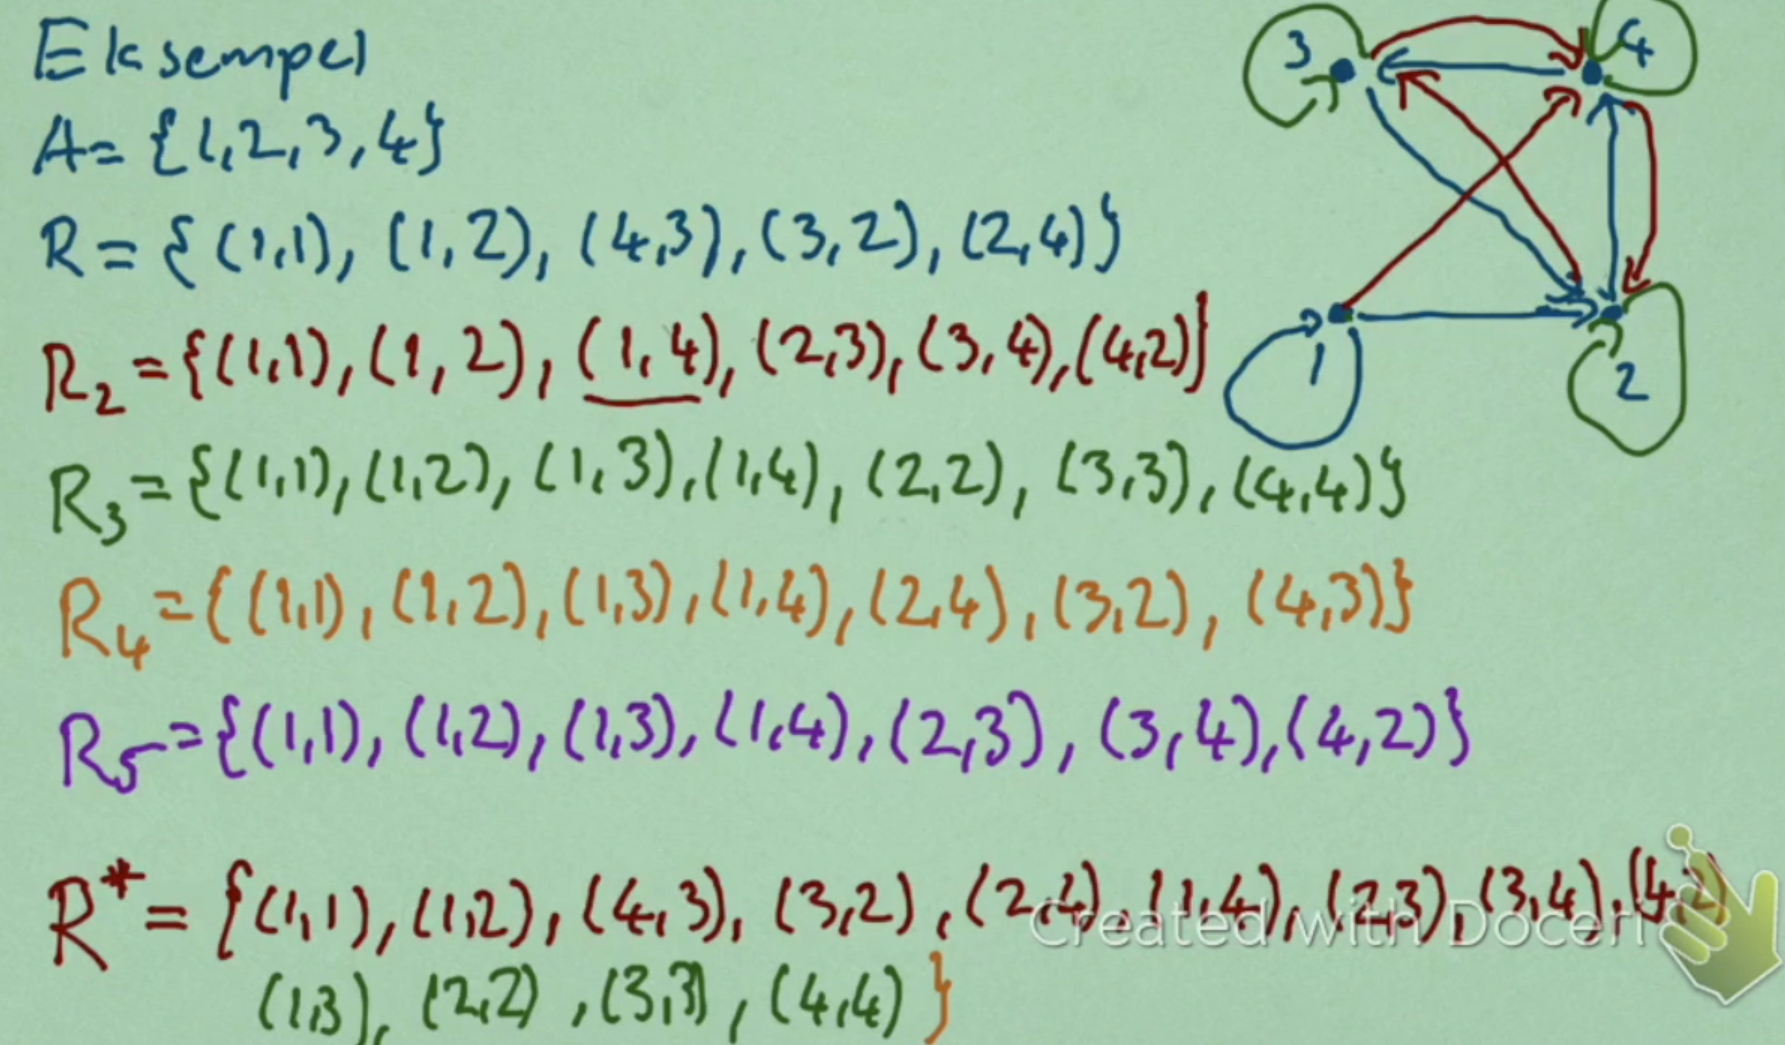
\includegraphics[keepaspectratio,scale=0.44593301435406696,height=6.472222222222222in]{workshop1_image1.png}}}\end{Maple Normal}
\begin{Maple Normal}{
\mapleinline{inert}{2d}{}{\[\]}
}\end{Maple Normal}
\subsubsection{\textbf{\textit{2. }}}
\begin{Maple Normal}{
\textbf{Opskriv den omtalte aflukning for relationen i Figur 1. Dette er en ny\linebreak
}\textbf{relation, som vi kalder S.}}\end{Maple Normal}

\begin{Maple Normal}{
Denne kan konstrueres med følgende formel \mapleinline{inert}{2d}{Typesetting:-mrow(Typesetting:-msup(Typesetting:-mi("R", italic = "true", mathvariant = "italic"), Typesetting:-mrow(Typesetting:-mo("*", mathvariant = "normal", fence = "false", separator = "false", stretchy = "false", symmetric = "false", largeop = "false", movablelimits = "false", accent = "false", lspace = "0.1666667em", rspace = "0.1666667em")), superscriptshift = "0"), Typesetting:-mo("=", mathvariant = "normal", fence = "false", separator = "false", stretchy = "false", symmetric = "false", largeop = "false", movablelimits = "false", accent = "false", lspace = "0.2777778em", rspace = "0.2777778em"), Typesetting:-mo("+", mathvariant = "normal", fence = "false", separator = "false", stretchy = "false", symmetric = "false", largeop = "false", movablelimits = "false", accent = "false", lspace = "0.2222222em", rspace = "0.2222222em"), Typesetting:-munderover(Typesetting:-mrow(Typesetting:-mo("&bigcup;", executable = "false", mathvariant = "normal", fence = "false", separator = "false", stretchy = "true", symmetric = "false", largeop = "true", movablelimits = "true", accent = "false", lspace = "0.0em", rspace = "0.1666667em")), Typesetting:-mrow(Typesetting:-mi("i", italic = "true", foreground = "[200,0,200]", placeholder = "true", mathvariant = "italic"), Typesetting:-mo("=", mathvariant = "normal", fence = "false", separator = "false", stretchy = "false", symmetric = "false", largeop = "false", movablelimits = "false", accent = "false", lspace = "0.2777778em", rspace = "0.2777778em"), Typesetting:-mn("1", mathvariant = "normal")), Typesetting:-mrow(Typesetting:-mo("&infin;", mathvariant = "normal", fence = "false", separator = "false", stretchy = "false", symmetric = "false", largeop = "false", movablelimits = "false", accent = "false", lspace = "0.0em", rspace = "0.0em")), accent = "false", accentunder = "false"), Typesetting:-msup(Typesetting:-mi("R", italic = "true", mathvariant = "italic"), Typesetting:-mrow(Typesetting:-mi("i", italic = "true", mathvariant = "italic")), superscriptshift = "0"))}{$\displaystyle R ^{*}=+\Mapleoverset{\infty }{\Mapleunderset{i =1}{\bigcup }}R ^{i }$}
. Man kan dog nøjes med kun at gøre det op til |A|, som i dette tilfælde er 7.}\end{Maple Normal}

\begin{Maple Normal}{
\mapleinline{inert}{2d}{R = {Bob, Gry, Kim, Liv, Mia, Noa, Tom, (Mia, Mia)*(Mia, Liv)}}{\[\]}
}\end{Maple Normal}
\begin{Maple Normal}{
\mapleinline{inert}{2d}{R^2 = {Bob, Gry, Kim, Liv, Mia, Noa, Tom, (Mia, Mia)*(Mia, Liv)}}{\[\]}
}\end{Maple Normal}
\begin{Maple Normal}{
\mapleinline{inert}{2d}{R^3 = {Bob, Gry, Kim, Liv, Mia, Noa, Tom, (Mia, Mia)*(Mia, Liv)}}{\[\]}
}\end{Maple Normal}
\begin{Maple Normal}{
\mapleinline{inert}{2d}{R^3 = R^4 and R^4 = R^5 and R^5 = R^6 and R^6 = R^7 and R^7 = R^%H and R^%H = S}{\[{R}^{3}={R}^{4} \land {R}^{4}={R}^{5} \land {R}^{5}={R}^{6}\\
\mbox{} \land {R}^{6}={R}^{7}\\
\mbox{} \land {R}^{7}={R}^{\mbox {{\tt `\%H`}}}\\
\mbox{} \land {R}^{\mbox {{\tt `\%H`}}}=S\]}
}\end{Maple Normal}
\begin{Maple Normal}{
\mapleinline{inert}{2d}{}{\[\]}
}\end{Maple Normal}
\subsection{\textbf{Delopgave 3}}
\subsubsection{\textbf{\textit{1.}}}
\begin{Maple Normal}{
\textbf{Betragt nu følgende mængder}}\end{Maple Normal}

\begin{Maple Normal}{
\textbf{}}\end{Maple Normal}
\begin{Maple Normal}{
\mapleinline{inert}{2d}{Typesetting:-mrow(Typesetting:-mi("`F__Tom`"), Typesetting:-mo("=", bold = "true", mathvariant = "bold", fontweight = "bold", fence = "false", separator = "false", stretchy = "false", symmetric = "false", largeop = "false", movablelimits = "false", accent = "false", lspace = "0.2777778em", rspace = "0.2777778em"), Typesetting:-mo("{", bold = "true", mathvariant = "bold", fontweight = "bold", fence = "true", separator = "false", stretchy = "true", symmetric = "false", largeop = "false", movablelimits = "false", accent = "false", lspace = "0.1666667em", rspace = "0.1666667em"), Typesetting:-mi("a", bold = "true", italic = "true", mathvariant = "bold-italic", fontweight = "bold"), Typesetting:-mo(" ", bold = "true", mathvariant = "bold", fontweight = "bold", fence = "false", separator = "false", stretchy = "false", symmetric = "false", largeop = "false", movablelimits = "false", accent = "false", lspace = "0.0em", rspace = "0.0em"), Typesetting:-mo("&in;", bold = "true", mathvariant = "bold", fontweight = "bold", fence = "false", separator = "false", stretchy = "false", symmetric = "false", largeop = "false", movablelimits = "false", accent = "false", lspace = "0.2777778em", rspace = "0.2777778em"), Typesetting:-mi("A", bold = "true", italic = "true", mathvariant = "bold-italic", fontweight = "bold"), Typesetting:-mo(" ", bold = "true", mathvariant = "bold", fontweight = "bold", fence = "false", separator = "false", stretchy = "false", symmetric = "false", largeop = "false", movablelimits = "false", accent = "false", lspace = "0.0em", rspace = "0.0em"), Typesetting:-mo("|", bold = "true", mathvariant = "bold", fontweight = "bold", fence = "false", separator = "false", stretchy = "true", symmetric = "false", largeop = "false", movablelimits = "false", accent = "false", lspace = "0.1111111em", rspace = "0.1111111em"), Typesetting:-mo(" ", bold = "true", mathvariant = "bold", fontweight = "bold", fence = "false", separator = "false", stretchy = "false", symmetric = "false", largeop = "false", movablelimits = "false", accent = "false", lspace = "0.0em", rspace = "0.0em"), Typesetting:-mfenced(Typesetting:-mrow(Typesetting:-mi("a", bold = "true", italic = "true", mathvariant = "bold-italic", fontweight = "bold"), Typesetting:-mo(",", bold = "true", mathvariant = "bold", fontweight = "bold", fence = "false", separator = "true", stretchy = "false", symmetric = "false", largeop = "false", movablelimits = "false", accent = "false", lspace = "0.0em", rspace = "0.3333333em"), Typesetting:-mi("Tom", bold = "true", italic = "true", mathvariant = "bold-italic", fontweight = "bold")), bold = "true", mathvariant = "bold", fontweight = "bold"), Typesetting:-mo(" ", bold = "true", mathvariant = "bold", fontweight = "bold", fence = "false", separator = "false", stretchy = "false", symmetric = "false", largeop = "false", movablelimits = "false", accent = "false", lspace = "0.0em", rspace = "0.0em"), Typesetting:-mo("&in;", bold = "true", mathvariant = "bold", fontweight = "bold", fence = "false", separator = "false", stretchy = "false", symmetric = "false", largeop = "false", movablelimits = "false", accent = "false", lspace = "0.2777778em", rspace = "0.2777778em"), Typesetting:-mi("S", bold = "true", italic = "true", mathvariant = "bold-italic", fontweight = "bold"), Typesetting:-mo("}", bold = "true", mathvariant = "bold", fontweight = "bold", fence = "true", separator = "false", stretchy = "true", symmetric = "false", largeop = "false", movablelimits = "false", accent = "false", lspace = "0.1666667em", rspace = "0.1111111em"))}{\[{\it `F__Tom` }=\left{a \mathop{\rm  }\in A \mathop{\rm  }\mid \mathop{\rm  }\left(a ,{\it Tom} \right)\mathop{\rm  }\in S \right}\]}
}\end{Maple Normal}
\begin{Maple Normal}{
\mapleinline{inert}{2d}{Typesetting:-mrow(Typesetting:-mi("`F__Noa`"), Typesetting:-mo("=", bold = "true", mathvariant = "bold", fontweight = "bold", fence = "false", separator = "false", stretchy = "false", symmetric = "false", largeop = "false", movablelimits = "false", accent = "false", lspace = "0.2777778em", rspace = "0.2777778em"), Typesetting:-mo("{", bold = "true", mathvariant = "bold", fontweight = "bold", fence = "true", separator = "false", stretchy = "true", symmetric = "false", largeop = "false", movablelimits = "false", accent = "false", lspace = "0.1666667em", rspace = "0.1666667em"), Typesetting:-mi("a", bold = "true", italic = "true", mathvariant = "bold-italic", fontweight = "bold"), Typesetting:-mo(" ", bold = "true", mathvariant = "bold", fontweight = "bold", fence = "false", separator = "false", stretchy = "false", symmetric = "false", largeop = "false", movablelimits = "false", accent = "false", lspace = "0.0em", rspace = "0.0em"), Typesetting:-mo("&in;", bold = "true", mathvariant = "bold", fontweight = "bold", fence = "false", separator = "false", stretchy = "false", symmetric = "false", largeop = "false", movablelimits = "false", accent = "false", lspace = "0.2777778em", rspace = "0.2777778em"), Typesetting:-mi("A", bold = "true", italic = "true", mathvariant = "bold-italic", fontweight = "bold"), Typesetting:-mo(" ", bold = "true", mathvariant = "bold", fontweight = "bold", fence = "false", separator = "false", stretchy = "false", symmetric = "false", largeop = "false", movablelimits = "false", accent = "false", lspace = "0.0em", rspace = "0.0em"), Typesetting:-mo("|", bold = "true", mathvariant = "bold", fontweight = "bold", fence = "false", separator = "false", stretchy = "true", symmetric = "false", largeop = "false", movablelimits = "false", accent = "false", lspace = "0.1111111em", rspace = "0.1111111em"), Typesetting:-mo(" ", bold = "true", mathvariant = "bold", fontweight = "bold", fence = "false", separator = "false", stretchy = "false", symmetric = "false", largeop = "false", movablelimits = "false", accent = "false", lspace = "0.0em", rspace = "0.0em"), Typesetting:-mfenced(Typesetting:-mrow(Typesetting:-mi("a", bold = "true", italic = "true", mathvariant = "bold-italic", fontweight = "bold"), Typesetting:-mo(",", bold = "true", mathvariant = "bold", fontweight = "bold", fence = "false", separator = "true", stretchy = "false", symmetric = "false", largeop = "false", movablelimits = "false", accent = "false", lspace = "0.0em", rspace = "0.3333333em"), Typesetting:-mi("Noa", bold = "true", italic = "true", mathvariant = "bold-italic", fontweight = "bold")), bold = "true", mathvariant = "bold", fontweight = "bold"), Typesetting:-mo(" ", bold = "true", mathvariant = "bold", fontweight = "bold", fence = "false", separator = "false", stretchy = "false", symmetric = "false", largeop = "false", movablelimits = "false", accent = "false", lspace = "0.0em", rspace = "0.0em"), Typesetting:-mo("&in;", bold = "true", mathvariant = "bold", fontweight = "bold", fence = "false", separator = "false", stretchy = "false", symmetric = "false", largeop = "false", movablelimits = "false", accent = "false", lspace = "0.2777778em", rspace = "0.2777778em"), Typesetting:-mi("S", bold = "true", italic = "true", mathvariant = "bold-italic", fontweight = "bold"), Typesetting:-mo("}", bold = "true", mathvariant = "bold", fontweight = "bold", fence = "true", separator = "false", stretchy = "true", symmetric = "false", largeop = "false", movablelimits = "false", accent = "false", lspace = "0.1666667em", rspace = "0.1111111em"))}{\[{\it `F__Noa` }=\left{a \mathop{\rm  }\in A \mathop{\rm  }\mid \mathop{\rm  }\left(a ,{\it Noa} \right)\mathop{\rm  }\in S \right}\]}
}\end{Maple Normal}
\begin{Maple Normal}{
\textbf{}}\end{Maple Normal}
\begin{Maple Normal}{
\textbf{Hvad beskriver mængderne? Hvilke elementer indeholder }\mapleinline{inert}{2d}{F__Tom, F__Noa}{$\displaystyle F_{{\it Tom}},\,F_{{\it Noa}}$}
\textbf{ og }\mapleinline{inert}{2d}{F__Tom intersect F__Noa}{$\displaystyle F_{{\it Tom}} \cap F_{{\it Noa}}$}
\textbf{.}}\end{Maple Normal}

\begin{Maple Normal}{
}\end{Maple Normal}
\begin{Maple Normal}{
Mængderne beskriver hvem der følger dem både direkte og indirekte.}\end{Maple Normal}

\begin{Maple Normal}{
\mapleinline{inert}{2d}{F__Tom = {Gry, Kim, Liv, Mia, Noa, Tom}}{\[F_{{\it Tom}}= \left\{ {\it Gry},{\it Kim},{\it Liv},{\it Mia}\\
\mbox{},{\it Noa},{\it Tom} \right\} \]}
}\end{Maple Normal}
\begin{Maple Normal}{
}\end{Maple Normal}
\begin{Maple Normal}{
\mapleinline{inert}{2d}{F__Noa = {Kim, Liv, Mia, Noa}}{$\displaystyle F_{{\it Noa}}= \left\{ {\it Kim},{\it Liv},{\it Mia},{\it Noa}\\
\mbox{} \right\} $}
\mapleinline{inert}{2d}{}{$\displaystyle $}
}\end{Maple Normal}
\begin{Maple Normal}{
\mapleinline{inert}{2d}{}{\[\]}
}\end{Maple Normal}
\begin{Maple Normal}{
\mapleinline{inert}{2d}{F__Tom intersect F__Noa = {Gry, Kim, Liv, Mia, Noa, Tom}}{\[F_{{\it Tom}} \cap F_{{\it Noa}}\\
\mbox{}= \left\{ {\it Gry},{\it Kim},{\it Liv},{\it Mia},{\it Noa}\\
\mbox{},{\it Tom} \right\} \]}
}\end{Maple Normal}
\begin{Maple Normal}{
\mapleinline{inert}{2d}{}{\[\]}
}\end{Maple Normal}
\subsubsection{\textbf{\textit{2.}}}
\begin{Maple Normal}{
\textbf{Lad }\mapleinline{inert}{2d}{B subset A}{$\displaystyle B \subseteq A$}
\textbf{ og betragt }\mapleinline{inert}{2d}{Typesetting:-mrow(Typesetting:-mi("`G__Tom`"), Typesetting:-mo("=", bold = "true", mathvariant = "bold", fontweight = "bold", fence = "false", separator = "false", stretchy = "false", symmetric = "false", largeop = "false", movablelimits = "false", accent = "false", lspace = "0.2777778em", rspace = "0.2777778em"), Typesetting:-mo("{", bold = "true", mathvariant = "bold", fontweight = "bold", fence = "true", separator = "false", stretchy = "true", symmetric = "false", largeop = "false", movablelimits = "false", accent = "false", lspace = "0.1666667em", rspace = "0.1666667em"), Typesetting:-mi("b", bold = "true", italic = "true", mathvariant = "bold-italic", fontweight = "bold"), Typesetting:-mo(" ", bold = "true", mathvariant = "bold", fontweight = "bold", fence = "false", separator = "false", stretchy = "false", symmetric = "false", largeop = "false", movablelimits = "false", accent = "false", lspace = "0.0em", rspace = "0.0em"), Typesetting:-mo("&in;", bold = "true", mathvariant = "bold", fontweight = "bold", fence = "false", separator = "false", stretchy = "false", symmetric = "false", largeop = "false", movablelimits = "false", accent = "false", lspace = "0.2777778em", rspace = "0.2777778em"), Typesetting:-mi("B", bold = "true", italic = "true", mathvariant = "bold-italic", fontweight = "bold"), Typesetting:-mo(" ", bold = "true", mathvariant = "bold", fontweight = "bold", fence = "false", separator = "false", stretchy = "false", symmetric = "false", largeop = "false", movablelimits = "false", accent = "false", lspace = "0.0em", rspace = "0.0em"), Typesetting:-mo("|", bold = "true", mathvariant = "bold", fontweight = "bold", fence = "false", separator = "false", stretchy = "true", symmetric = "false", largeop = "false", movablelimits = "false", accent = "false", lspace = "0.1111111em", rspace = "0.1111111em"), Typesetting:-mo(" ", bold = "true", mathvariant = "bold", fontweight = "bold", fence = "false", separator = "false", stretchy = "false", symmetric = "false", largeop = "false", movablelimits = "false", accent = "false", lspace = "0.0em", rspace = "0.0em"), Typesetting:-mfenced(Typesetting:-mrow(Typesetting:-mi("b", bold = "true", italic = "true", mathvariant = "bold-italic", fontweight = "bold"), Typesetting:-mo(",", bold = "true", mathvariant = "bold", fontweight = "bold", fence = "false", separator = "true", stretchy = "false", symmetric = "false", largeop = "false", movablelimits = "false", accent = "false", lspace = "0.0em", rspace = "0.3333333em"), Typesetting:-mi("Tom", italic = "true", mathvariant = "italic")), mathvariant = "normal"), Typesetting:-mo("&in;", mathvariant = "normal", fence = "false", separator = "false", stretchy = "false", symmetric = "false", largeop = "false", movablelimits = "false", accent = "false", lspace = "0.2777778em", rspace = "0.2777778em"), Typesetting:-mi("S", bold = "true", italic = "true", mathvariant = "bold-italic", fontweight = "bold"), Typesetting:-mo("}", mathvariant = "normal", fence = "true", separator = "false", stretchy = "true", symmetric = "false", largeop = "false", movablelimits = "false", accent = "false", lspace = "0.1666667em", rspace = "0.1111111em"))}{$\displaystyle {\it `G__Tom` }=\left{b \mathop{\rm  }\in B \mathop{\rm  }\mid \mathop{\rm  }\left(b ,{\it Tom} \right)\in S \right}$}
\textbf{. Vis, at }}\end{Maple Normal}

\begin{Maple Normal}{
\mapleinline{inert}{2d}{G__Tom subset F__Tom}{$\displaystyle G_{{\it Tom}} \subseteq F_{{\it Tom}}$}
\textbf{.}}\end{Maple Normal}

\begin{Maple Normal}{
\mapleinline{inert}{2d}{}{\[\]}
}\end{Maple Normal}
\begin{Maple Normal}{
\mapleinline{inert}{2d}{Typesetting:-mrow(Typesetting:-mi("`G__Tom`"), Typesetting:-mo("=", font_style_name = "2D Input", mathvariant = "normal", fence = "false", separator = "false", stretchy = "false", symmetric = "false", largeop = "false", movablelimits = "false", accent = "false", lspace = "0.2777778em", rspace = "0.2777778em"), Typesetting:-mo("{", font_style_name = "2D Input", mathvariant = "normal", fence = "true", separator = "false", stretchy = "true", symmetric = "false", largeop = "false", movablelimits = "false", accent = "false", lspace = "0.1666667em", rspace = "0.1666667em"), Typesetting:-mi("b", italic = "true", font_style_name = "2D Input", mathvariant = "italic"), Typesetting:-mo(" ", font_style_name = "2D Input", mathvariant = "normal", fence = "false", separator = "false", stretchy = "false", symmetric = "false", largeop = "false", movablelimits = "false", accent = "false", lspace = "0.0em", rspace = "0.0em"), Typesetting:-mo("&in;", font_style_name = "2D Input", mathvariant = "normal", fence = "false", separator = "false", stretchy = "false", symmetric = "false", largeop = "false", movablelimits = "false", accent = "false", lspace = "0.2777778em", rspace = "0.2777778em"), Typesetting:-mi("B", italic = "true", font_style_name = "2D Input", mathvariant = "italic"), Typesetting:-mo(" ", font_style_name = "2D Input", mathvariant = "normal", fence = "false", separator = "false", stretchy = "false", symmetric = "false", largeop = "false", movablelimits = "false", accent = "false", lspace = "0.0em", rspace = "0.0em"), Typesetting:-mo("|", font_style_name = "2D Input", mathvariant = "normal", fence = "false", separator = "false", stretchy = "true", symmetric = "false", largeop = "false", movablelimits = "false", accent = "false", lspace = "0.1111111em", rspace = "0.1111111em"), Typesetting:-mo(" ", font_style_name = "2D Input", mathvariant = "normal", fence = "false", separator = "false", stretchy = "false", symmetric = "false", largeop = "false", movablelimits = "false", accent = "false", lspace = "0.0em", rspace = "0.0em"), Typesetting:-mfenced(Typesetting:-mrow(Typesetting:-mi("b", italic = "true", font_style_name = "2D Input", mathvariant = "italic"), Typesetting:-mo(",", font_style_name = "2D Input", mathvariant = "normal", fence = "false", separator = "true", stretchy = "false", symmetric = "false", largeop = "false", movablelimits = "false", accent = "false", lspace = "0.0em", rspace = "0.3333333em"), Typesetting:-mi("Tom", italic = "true", font_style_name = "2D Input", mathvariant = "italic")), font_style_name = "2D Input", mathvariant = "normal"), Typesetting:-mo("&in;", font_style_name = "2D Input", mathvariant = "normal", fence = "false", separator = "false", stretchy = "false", symmetric = "false", largeop = "false", movablelimits = "false", accent = "false", lspace = "0.2777778em", rspace = "0.2777778em"), Typesetting:-mi("S", italic = "true", font_style_name = "2D Input", mathvariant = "italic"), Typesetting:-mo("}", font_style_name = "2D Input", mathvariant = "normal", fence = "true", separator = "false", stretchy = "true", symmetric = "false", largeop = "false", movablelimits = "false", accent = "false", lspace = "0.1666667em", rspace = "0.1111111em"), Typesetting:-mo("&subseteq;", font_style_name = "2D Input", mathvariant = "normal", fence = "false", separator = "false", stretchy = "false", symmetric = "false", largeop = "false", movablelimits = "false", accent = "false", lspace = "0.2777778em", rspace = "0.2777778em"), Typesetting:-mo("{", font_style_name = "2D Input", mathvariant = "normal", fence = "true", separator = "false", stretchy = "true", symmetric = "false", largeop = "false", movablelimits = "false", accent = "false", lspace = "0.1666667em", rspace = "0.1666667em"), Typesetting:-mi("a", italic = "true", font_style_name = "2D Input", mathvariant = "italic"), Typesetting:-mo(" ", font_style_name = "2D Input", mathvariant = "normal", fence = "false", separator = "false", stretchy = "false", symmetric = "false", largeop = "false", movablelimits = "false", accent = "false", lspace = "0.0em", rspace = "0.0em"), Typesetting:-mo("&in;", font_style_name = "2D Input", mathvariant = "normal", fence = "false", separator = "false", stretchy = "false", symmetric = "false", largeop = "false", movablelimits = "false", accent = "false", lspace = "0.2777778em", rspace = "0.2777778em"), Typesetting:-mi("A", italic = "true", font_style_name = "2D Input", mathvariant = "italic"), Typesetting:-mo(" ", font_style_name = "2D Input", mathvariant = "normal", fence = "false", separator = "false", stretchy = "false", symmetric = "false", largeop = "false", movablelimits = "false", accent = "false", lspace = "0.0em", rspace = "0.0em"), Typesetting:-mo("|", font_style_name = "2D Input", mathvariant = "normal", fence = "false", separator = "false", stretchy = "true", symmetric = "false", largeop = "false", movablelimits = "false", accent = "false", lspace = "0.1111111em", rspace = "0.1111111em"), Typesetting:-mo(" ", font_style_name = "2D Input", mathvariant = "normal", fence = "false", separator = "false", stretchy = "false", symmetric = "false", largeop = "false", movablelimits = "false", accent = "false", lspace = "0.0em", rspace = "0.0em"), Typesetting:-mfenced(Typesetting:-mrow(Typesetting:-mi("a", italic = "true", font_style_name = "2D Input", mathvariant = "italic"), Typesetting:-mo(",", font_style_name = "2D Input", mathvariant = "normal", fence = "false", separator = "true", stretchy = "false", symmetric = "false", largeop = "false", movablelimits = "false", accent = "false", lspace = "0.0em", rspace = "0.3333333em"), Typesetting:-mi("Tom", italic = "true", font_style_name = "2D Input", mathvariant = "italic")), font_style_name = "2D Input", mathvariant = "normal"), Typesetting:-mo(" ", font_style_name = "2D Input", mathvariant = "normal", fence = "false", separator = "false", stretchy = "false", symmetric = "false", largeop = "false", movablelimits = "false", accent = "false", lspace = "0.0em", rspace = "0.0em"), Typesetting:-mo("&in;", font_style_name = "2D Input", mathvariant = "normal", fence = "false", separator = "false", stretchy = "false", symmetric = "false", largeop = "false", movablelimits = "false", accent = "false", lspace = "0.2777778em", rspace = "0.2777778em"), Typesetting:-mi("S", italic = "true", font_style_name = "2D Input", mathvariant = "italic"), Typesetting:-mo("}", font_style_name = "2D Input", mathvariant = "normal", fence = "true", separator = "false", stretchy = "true", symmetric = "false", largeop = "false", movablelimits = "false", accent = "false", lspace = "0.1666667em", rspace = "0.1111111em"))}{\[{\it `G__Tom` }=\left{b \mathop{\rm  }\in B \mathop{\rm  }\mid \mathop{\rm  }\left(b ,{\it Tom} \right)\in S \right}\subseteq \left{a \mathop{\rm  }\in A \mathop{\rm  }\mid \mathop{\rm  }\left(a ,{\it Tom} \right)\mathop{\rm  }\in S \right}\]}
}\end{Maple Normal}
\begin{Maple Normal}{
Mængderne afhenger af to andre mængder, men eller er de fuldstænig ens. siden \mapleinline{inert}{2d}{B subset A}{$\displaystyle B \subseteq A$}
 kan du højst have lige mange mulige i \mapleinline{inert}{2d}{G__Tom}{$\displaystyle G_{{\it Tom}}$}
 da alle de matches du har i \mapleinline{inert}{2d}{G__Tom}{$\displaystyle G_{{\it Tom}}$}
 også er matches i \mapleinline{inert}{2d}{F__Tom}{$\displaystyle F_{{\it Tom}}$}
.}\end{Maple Normal}

\begin{Maple Normal}{
\mapleinline{inert}{2d}{}{\[\]}
}\end{Maple Normal}
\begin{Maple Normal}{
\mapleinline{inert}{2d}{}{\[\]}
}\end{Maple Normal}
\begin{Maple Normal}{
\mapleinline{inert}{2d}{}{\[\]}
}\end{Maple Normal}
\begin{Maple Normal}{
\mapleinline{inert}{2d}{}{$\displaystyle $}
\mapleinline{inert}{2d}{}{$\displaystyle $}
\mapleinline{inert}{2d}{}{$\displaystyle $}
}\end{Maple Normal}
\begin{Maple Normal}{
\mapleinline{inert}{2d}{}{\[\]}
}\end{Maple Normal}
\end{document}
